\documentclass[11pt]{report}

\usepackage[utf8]{inputenc}
\usepackage[T1]{fontenc}
\usepackage[spanish]{babel}
\usepackage{times}
\usepackage{listings}
\usepackage{color}
\usepackage{float}

\usepackage[colorlinks=true,linkcolor=blue,urlcolor=blue]{hyperref}

\usepackage{fancyhdr}

% paragraphs 
\usepackage{titlesec}
\titleformat{\paragraph}
    {\normalfont\bfseries}
    {}
    {0pt}
    {}
\titleformat{\subparagraph}
    {\normalfont\bfseries}
    {}
    {0pt}
    {}
    
\usepackage{wasysym}

%%%%% margenes
\usepackage{anysize}
\marginsize{3cm}{2cm}{2cm}{2cm}

\addto\captionsspanish{\renewcommand{\chaptername}{Sección}}

% para los itemize anidados
\renewcommand{\labelitemi}{$\bullet$}
\renewcommand{\labelitemii}{$\cdot$}
\renewcommand{\labelitemiii}{$\diamond$}
\renewcommand{\labelitemiv}{$\ast$}

% para los enum anidados
\renewcommand{\labelenumi}{\arabic{enumi}. }
\renewcommand{\labelenumii}{\labelenumi\alph{enumii}) }
\renewcommand{\labelenumiii}{\labelenumii\roman{enumiii}: }

%\includeonly{Memoria}


\setcounter{secnumdepth}{4} % how many sectioning levels to assign numbers to
\setcounter{tocdepth}{4}


\title{\textbf{Titulo}}
\author{César Antonio Enrique Ramírez}
\date{\today}

%//////////////// Documento //////////////////////%
\usepackage{graphicx}
\begin{document}

\maketitle
\tableofcontents
\newpage

\thispagestyle{empty}
\null
\vfill
\begin{center}
	Esta página fue dejada en blaco a propósito.
\end{center}
\newpage

\section*{INTRODUCCIÓN.}
\addcontentsline{toc}{section}{INTRODUCCIÓN}

La redacción del proyecto correspode a los alumnos Alejandro Trujillo Caballero, Andrés Jesús díaz santos y César Antonio Enrique Ramírez. El proyecto a llevar a cabo comprende 10 edificios unifamiliares de 2 plantas y un local de 100 m\pow{2}. 
\chapter{MEMORIA.}

\section{DATOS GENERALES.}

\subsection{Descripción del edificio o complejo urbano, con indicación del número de bloques, portales, escaleras, plantas, viviendas por planta, dependencias de cada vivienda, locales comerciales, oficinas, etc.}
\subsection{Aplicación de la Ley de la Propiedad Horizontal.}
\subsection{Objeto del Proyecto Técnico.}
Dar cumplimiento al Real Decreto-ley 1/1.998 de 27 de Febrero sobre infraestructuras comunes en los
edificios para el acceso a los servicios de telecomunicaciones y establecer los condicionantes
técnicos que debe cumplir la instalación de ICT, de acuerdo con el Real Decreto 346/2011, de 11 de marzo, relativo al Reglamento regulador de las infraestructuras comunes de edificios y a la Roden ITC/1644/2011, de 10 de junio, del Ministerio de Industria Turismo y Comercio, que desarrolla el citado Reglamento.
Así mismo se dará cumplimiento a la LEY 10/2005, de 14 de junio (BOE 15/06/2005), de medidas urgentes para el impulso de la Televisión Digital Terrestre, de liberalización de la televisión por cable y de fomento del pluralismo.

La infraestructura común de telecomunicaciones consta de los elementos necesarios para satisfacer inicialmente las siguientes funciones:

\begin{itemize}
	\item La captación y adaptación de las señales digitales, terrestres, de radiodifusión sonora y televisión y su distribución hasta puntos de conexión situados en las distintas viviendas o locales de las edificaciones, y la distribución de las señales, por satétlite, de radiodifusión sonora y televisión hasta los citados puntos de conexión.
	\item Proporcionar el acceso a los servicios de telefonía disponible al público (STDP) y a los servicios de telecomunicaciones de banda ancha prestados a través de redes pñublicas de comunicaciones electrónicas por operadores habilitados para el establecimiento y explotación de las mismas, mediante la infraestructura necesaria que permita la conexión de las distintas viviendas o locales a las redes de los operadores habilitados.
\end{itemize}

La iCt está sustentada por la infraestructura de canalizaciones dimensionada según el Anexo III del Real Decreto 346/2011, que garantiza la posibilidad de incorporación de nuevos servicios que puedan surgir en un próximo futuro.

Se ha establecido un plan de frecuencias para la distribución de las señales de televisión y radiodifusión terrestre de las entidades con título habilitante que, sin manipulación ni conversión de frecuencias, permita la distribución de señales no contempladas en la instalación inicial por los canales previstos, de forma que no se afecten los servicios existentes y se respeten los canales destinados a otros servicios que puedan incorporarse en un futuro. La desaparición de la TV analógica y la incorporación de la TV digital terrestre conlleva el uso de las frecuencias 195.0 MHz a 223.0 MHz (C8 a C11, BIII) y 470 MHz a 862 MHz (C21 a C69, BIV y BV), que se destinarán con carácter prioritario, para la distribución de señales de radiodifusión sonora digital y televisión digital terrestre.



\section{ELEMENTOS QUE CONSTITUYEN LA INFRAESTRUCTURA COMÚN DE TELECOMUNICACIÓN.}

\subsection{Captación y distribución de radiodifusión sonora y televisión terrestres.}

\subsubsection{Consideraciones sobre el Diseño.}


Las antenas para la recepción de las señales de radiodifusión terrestre y recepción satélite se instalarán sobre el tejado del RITU (ver planos \ref{} AÑADIR REFERENCIA).

Se utilizarán cinco antenas, dos para satélite, dos para radio (Satelite, VHF y Terrestre, FM B-II) y una para televisión.

Los canales serán amplificados en cabecera mediante amplificadores monocanales con objeto de evitar la intermodulación entre ellos. Su figura de ruido, ganancia y nivel máximo de salida se han seleccionado para garantizar en las tomas de usuarios los niveles de calidad exigidos por el Real Decreto 346/2011. Con objeto de reducir el volumen, peso y coste de la cabecera terrestre, los
cuatro canales adyacentes del servicio DAB y los cuatro digitales más elevados (canales 66 a 69), también adyacentes, serán amplificados mediante sendos amplificadores de grupo.

Las redes de distribución y dispersión se han diseñado para obtener el mayor equilibrio posible entre las distintas tomas de usuario con los elementos de red establecidos en el correspondiente apartado del pliego de condiciones.

Siguiendo lo establecido en el Anexo I del Real Decreto 346/2011 las redes de TV se han diseñado con una estructura en estrella colocando a la salida del PAU un distribuidor de tantas vías como estancias (sin incluir baños y trasteros) existen en la vivienda.

El promotor ha definido la existencia de un local comercial pero sin facilitar la distribución interior. Puesto que se carece de esa información se equipará un PAU pero no se instalará distribuidor ni tomas.

\subsubsection{Número de tomas.}

\begin{table}[H]
\caption{Número de tomas de RTV}
\label{tomasRTV}
\begin{center}
\begin{tabular}{|c|c|c|}
\hline
	 & Número de estancias/vivienda & Número de tomas\\
\hline
	Planta baja & 2 & 2\\
\hline
	Primera Planta & 5 & 5\\
\hline
    Local comercial & 0 & 0\\
\hline
\end{tabular}
\end{center}
\end{table}


\begin{table}[H]
\caption{Número total de tomas de RTV}
\label{tomasRTVtotal}
\begin{center}
\begin{tabular}{|c|c|}
\hline
    Total tomas en Viviendas & 70\\
\hline 
    Total tomas en locales comerciales & 0\\
\hline
    Total de tomas & 70	\\
\hline
\end{tabular}
\end{center}
\end{table}

El número total de tomas es de 70 en viviendas. No existen estancias comunes en la edificación.

Según lo dispuesto en el apartado 3.5.2 del Anexo I del Reglamento de ICT, en cada local se colocará un PAU capaz de alimentar un número de tomas fijado en función de la superficie o división interior del los locales. En nuestro caso al no estar definida la división interior, no se colocarán tomas. El diseño y dimensionamiento de la red interior de usuario, así como su instalación futura, será responsabilidad de la propiedad del local, cuando se ejecute el proyecto de su distribución en estancias.

\paragraph{Número de repartidores, derivadores, según su ubicación en la red, PAU y sus características, así como las de los cables utilizados.}

Las redes de distribución y dispersión están formadas por una estructura árbol-rama.
La red de distribución comienza a la salida del mezclador de señales terrestres y satélites y finaliza en el derivador del local.
Las redes interiores tendrán estructura de estrella.


\subparagraph*{Derivadores, PAUs y Repartidores interiores de viviendas y locales}

Cada dos viviendas se colocará un derivador de dos salidas.

En cada vivienda se colocará, a la salida del PAU un distribuidor de 7 salidas. 

A ellas se conectarán los cables de la red interior de usuario correspondientes a cada estancia.

En el local no se instalará distribuidor, instalándose únicamente el PAU.

\subparagraph*{Cables}

Se utilizará un cable de 7 mm de diámetro exterior que deberá cumplir la norma UNE-EN 50117-2-4.

Sus características se especifican en el Pliego de Condiciones.

\subparagraph*{Tomas}

En cada vivienda el número de tomas instaladas es de 7.

En el local comercial, no se instalarán tomas.

No hay estancias comunes en la edificación.

Las caráteristicas técnicas de todos estos elementos se incluyen en el Pliego de Condiciones.
\subsection{Distribución de radiodifusión sonora y televisión por satélite.}
\subsection{Acceso y distribución de los servicios de telecomunicaciones de telefonía disponible al público (STDP) y de banda ancha (TBA).}
\subsubsection{Redes de Distribución y Dispersión.}
Este capítulo tiene por objeto describir y detallar las características de la red que permitan el
acceso y la distribución de los servicios de telecomunicaciones de telefonía disponible al público y
de banda ancha.
Según se establece en el artículo 9 del Real Decreto 346/2011 en este proyecto se describirán y
proyectarán la totalidad de las redes que pueden formar parte de la ICT, de acuerdo a la
presencia de operadores que despliegan red en la ubicación de la futura edificación.
La instalación de la red será con Cables de Pares Trenzados y coaxiales.
\paragraph{Redes de cables de pares trenzados.}\textbf{}\\
Los cables de pares trenzados se utilizan en la red de distribución y
dispersión y en la red interior de usuario.
Para las redes de distribución y dispersión, los cables de pares trenzados
utilizados serán, como mínimo, de 4 pares de hilos conductores de cobre con
aislamiento individual sin apantallar clase E (categoría 6), deberán cumplir las
especificaciones de la norma UNE-EN 50288-6-1 (Cables metálicos con
elementos múltiples utilizados para la transmisión y el control de señales
analógicas y digitales. Parte Especificación intermedia para cables sin
apantallar aplicables hasta 250 MHz. Cables para instalaciones horizontales y
verticales en edificios).

Para la red interior de usuario, los cables utilizados serán como mínimo de
cuatro pares de hilos conductores de cobre con aislamiento individual clase E
(categoría 6) y cubierta de material no propagador de la llama, libre de
halógenos y baja emisión de humos, y deberán ser conformes a las
especificaciones de la norma UNE-EN 50288-6-1 (Cables metálicos con
elementos múltiples utilizados para la transmisión y el control de señales
analógicas y digitales. 
\subparagraph{Establecimiento de la topología de la red de cables de pares.}

\begin{itemize}
	\item \textbf{Red de alimentación}\\
	Los Operadores de los servicios de telecomunicaciones de telefonía disponible al público y de
	banda ancha, accederán al edificio a través de sus redes de alimentación, que pueden ser
	mediante cables o vía radio. En cualquier caso, accederán al Recinto de Instalaciones de
	Telecomunicación correspondiente y terminarán en unas regletas de conexión (Regletas de
	Entrada) situadas en el Registro Principal de cables de Pares situadas en el RITU.
	Hasta este punto es responsabilidad de cada operador el diseño, dimensionamiento e instalación
	de la red de alimentación. El acceso de la misma hasta el RITU se realizará a través de la arqueta
	de entrada, canalización externa y canalización de enlace.
	En el Registro Principal, se colocarán también las regletas o paneles de conexión desde las
	cuales partirán los cables que se distribuyen hasta cada usuario, además dispone de espacio
	suficiente para alojar las guías y soportes necesarios para el encaminamiento de cables y puentes
	así como para los paneles o regletas de entrada de los operadores.
	En el RITU también se establece una previsión de espacio para la eventual instalación de los equipos de
	recepción y procesado de la señal en el caso en que los operadores accedan vía radio.
	
\end{itemize}

\begin{itemize}
	\item \textbf{Red interior del edificio}\\
\textbf{Opción con Cable de Pares Trenzados}\\
Con el diseño del tendido de la red de distribución/dispersión de cables de pares trenzados
previsto en el presente proyecto, no se supera, en ningún caso, la longitud de 100 m entre el
registro principal y cualquiera de los PAU (según se puede comprobar en el correspondiente
esquema incluido en el apartado de Planos), por lo que se realizan las citadas redes mediante
cables de pares trenzados, de acuerdo a lo establecido en el apartado 3.1.1 del Anexo II del
Reglamento.\\
La red interior del edificio se compone de:\\
- Red de distribución/dispersión\\
- Red interior de usuario\\
La red total se refleja en el esquema presente en la sección \textbf{PLANOS.}\\
Las diferentes redes que constituyen la red total del edificio se conexionan entre sí en los puntos
siguientes:\\
- Punto de Interconexión (entre la red de alimentación y la red de distribución/dispersión)\\
- Punto de distribución (entre la red de distribución y la red de dispersión). En este caso no tiene implementación física en los registros secundarios ya que al ser la red de cables de pares trenzados en estrella, se dispondrá de un cable sin solución de continuidad desde el Registro Principal hasta cada PAU. El punto de distribución y de interconexión, coinciden en el Registro Principal.\\
- Punto de acceso de usuario (entre la red de dispersión y la red interior de usuario)\\

\end{itemize}

\subparagraph{Cálculo y dimensionamiento de las redes de distribución y dispersión de cables de pares trenzados y tipos de cables.}\textbf{}\\
El conjunto de 10 viviendas unifamiliares y el local comercial, objeto del presente
proyecto, tiene la siguiente distribución:\\
Planta baja:		2 estancias\\
Primera planta: 	5 estancias\\
Un local sin distribución interior en estancias.\\
No existe previsión de conjunto de oficinas.
\begin{itemize}
	\item \textbf{Opción con Cable de Pares Trenzados}\\
	El número de acometidas necesarias, cada una formada por un cable no apantallado de 4 pares trenzados de cobre de Categoría 6 Clase E es de:\\
	\begin{table}[H]
\centering
\begin{tabular}{|p{5cm}| p{5cm}| p{5cm}|}
\hline
""&NÚMERO DE PAU&NÚMERO DE CABLES DE 4 PARES TRENZADOS \\
\hline \hline
VIVIENDAS&10&10\\
\hline
LOCALES COMERCIALES&1&1\\
\hline
CABLES PREVISTOS&""&11\\
\hline
COEFICIENTE CORRECTOR&""&1.2\\
\hline
CONEXIONES NECESARIAS&""&13.2->14\\
\hline
CONEXIONES PREVISTAS&""&14\\
\hline
\end{tabular}

\caption{Cálculo nº acometidas}
\label{tabla:autores}
\end{table}

El número de cables necesarios es de 14 y corresponde a viviendas y locales de utilización permanente con una ocupación aproximada de la red del 80%.\\
No obstante y con la finalidad de que en cada vivienda exista al menos un cable de reserva para
posibles roturas o averías, se ha previsto instalar 14 cables.\\
Dado que la red de cables de pares trenzados es en estrella, los cables de esta red se tienden
directamente desde el punto de interconexión hasta el PAU de cada vivienda o local (11 en total,
uno para cada vivienda y local), y los 3 restantes quedarán finalizados uno en cada uno de los
registros secundarios de cada vivienda con holgura suficiente para llegar al RTR de la primera planta.\\
Así, la red de distribución y dispersión estará formada por 24 cables UTP de cobre de 4 pares categoría 6 Clase E.

\end{itemize}

\subparagraph{Estructura de distribución y conexión.}
\begin{itemize}
	\item \textbf{Opción con Cable de Pares Trenzados}\\
	Al local comercial llegan 2 cables de pares trenzados, quedando uno de reserva en el registro
secundario.\\
A cada vivienda llegarán 2 cables, quedando uno de reserva.\\
Estos cables se conectarán, en su extremo inferior, a los conectores RJ45 hembra del panel de
conexión situado en el Registro Principal de cables de Pares, instalado en el RITU, y en su
extremo superior finalizarán en la roseta (conector hembra RJ45) de cada vivienda y local salvo
los de reserva que quedarán almacenados en el registro secundario de la cada vivienda.\\
Los cables deberán estar etiquetados en ambos extremos, indicando en cada uno de ellos la
vivienda a la que se corresponde, incluidos los de reserva.
\end{itemize}

\subparagraph{Resumen de los materiales necesarios para la red de cables de pares.}
Las características de los todos materiales utilizados se indican en el Pliego de Condiciones.

\paragraph{Redes de cables coaxiales.}
\subparagraph{Establecimiento de la topología de la red de cables coaxiales.}
\begin{itemize}
	\item \textbf{Red de alimentación}\\
	Los Operadores de los servicios de telecomunicaciones de cable coaxial para servicios de banda
ancha, accederán a las viviendas a través de sus redes de alimentación. En cualquier caso, accederán
al Recinto de Instalaciones de Telecomunicación correspondiente y terminarán sus redes en unos
paneles de conexión o regletas de entrada situadas en el Registro Principal de Cables Coaxiales
situados en el RITU. Estos paneles de conexión estarán constituidos por derivadores o
repartidores terminados en conectores tipo F hembra.
Hasta este punto es responsabilidad de cada operador el diseño, dimensionamiento e instalación
de la red de alimentación. El acceso de la misma hasta el RITU se realizará a través de la arqueta
de entrada, canalización externa y canalización de enlace.
Del Registro Principal de Cables Coaxiales, partirán los propios cables de la red de distribución
de la edificación terminados con conectores tipo F macho, dotados con la coca suficiente como
para permitir posibles reconfiguraciones.
En el RITU se deberá hacer una previsión de espacio para el caso de que sea necesaria
amplificación, cuando el operador accede mediante cable.
En el RITU se establece una previsión de espacio para la eventual instalación de los equipos de
recepción y procesado de la señal en el caso en que los operadores accedan vía radio.
\end{itemize}
\begin{itemize}
	\item \textbf{Red interior del edificio}\\
Al tratarse de una infraestructura con menos de 20 PAUs, la configuración de la red debe seguir una topología en estrella.\\
Al no haber una distancia mayor de 100m entre RITU y PAU más alejado tenemos una pérdida menor a 20dB.\\
Todos los cables salen del registro principal.
En el PAU se incluirá un distribuidor inductivo de 2 salidas F simétricas.
Las diferentes redes que constituyen la red total del edificio se conexionan entre sí en los puntos
siguientes:\\
- Punto de Interconexión (entre la red de alimentación y la red de distribución).\\
- Punto de distribución (entre la red de distribución y la red de dispersión). En este caso no tiene
implementación física en los registros secundarios ya que al ser la red de cable coaxial en
estrella, se dispondrá de un cable sin solución de continuidad desde el Registro Principal hasta
cada PAU. El punto de distribución y de interconexión, coinciden en el Registro Principal.\\
- Punto de acceso de usuario (entre la red de dispersión y la red interior de usuario).\\
\end{itemize}
\subparagraph{Cálculo y dimensionamiento de las redes de distribución y dispersión de cables coaxiales y tipos de cables.}
La urbanización de 10 viviendas unifamiliares y un local comercial, objeto del presente proyecto, tiene la siguiente distribución:\\
Planta baja y Primera planta:			Dos plantas por vivienda\\
Planta baja:							Local comercial\\
El número de acometidas necesarias, constituida cada una por un cable coaxial del tipo RG 59 es de:
\begin{table}[H]
\centering
\begin{tabular}{|p{5cm} |p{5cm} |p{5cm}|}
\hline
""&NÚMERO DE PAU&NÚMERO DE CABLES COAXIALES \\
\hline \hline
VIVIENDAS&10&10\\
\hline
LOCALES COMERCIALES&1&1\\
\hline
CABLES PREVISTOS&""&11\\
\hline
CONEXIONES NECESARIAS&""&11\\
\hline
\end{tabular}
\caption{Cálculo nº acometidas coaxiales}
\label{tabla:autores}
\end{table}
No se instalan cables de reserva.\\
Por tanto la red de distribución-dispersión estará formada por 11 cables coaxiales del tipo RG 59.
\subparagraph{Estructura de distribución y conexión.}
Seguirá una topología en estrella con un número de 11 tomas, 10 para viviendas y una para el local comercial.\\
Las conectores macho tipo “F” serán los empleados.
\subparagraph{Resumen de los materiales necesarios para la red de cables coaxiales.}
Las características de los todos materiales utilizados se indican en el Pliego de Condiciones.
\paragraph{Redes de cables de fibra óptica.}
\subparagraph{Establecimiento de la topología de la red de cables de fibra óptica.}
\begin{itemize}
	\item \textbf{Red de Alimentación}\\
	Los Operadores de los servicios de telecomunicaciones de cable de fibra óptica para servicios de
banda ancha, accederán al edificio a través de sus redes de alimentación. En cualquier caso,
accederán al Recinto de Instalaciones de Telecomunicación correspondiente y terminarán sus
redes en unos paneles de conectores de entrada situados en el Registro Principal de Cables de
Fibra Óptica situados en el RITU.
Hasta este punto es responsabilidad de cada operador el diseño, dimensionamiento e instalación
de la red de alimentación. El acceso de la misma hasta el RITU se realizará a través de la arqueta
de entrada, canalización externa y canalización de enlace.
Del Registro Principal de Cable de Fibra Óptica, partirán los propios cables de la red de
distribución de la edificación terminados con conectores tipo SC/APC, dotados con la coca
suficiente como para permitir posibles reconfiguraciones.
\end{itemize}

\begin{itemize}
	\item \textbf{Red interior del edificio}\\
Al tratarse de una edificación con menos de 15 PAUs, la red de distribución y dispersión se hará
en estrella desde el Registro Principal.\\
Las diferentes redes que constituyen la red total del edificio se conexionan entre sí en los puntos
siguientes:\\
- Punto de Interconexión (entre la red de alimentación y la red de distribución).\\
- Punto de distribución (entre la red de distribución y la red de dispersión). En este caso no tiene
implementación física en los registros secundarios ya que al ser la red de cable de fibra óptica en
estrella, se dispondrá de un cable de dos fibras ópticas sin solución de continuidad desde el
Registro Principal de Cable de Fibra Óptica hasta cada PAU. El punto de distribución y de
interconexión, coinciden en el Registro Principal de Cable de Fibra Óptica.\\
- Punto de acceso de usuario.\\
\end{itemize}
\subparagraph{Cálculo y dimensionamiento de las redes de distribución y dispersión de cables de fibra óptica y tipos de cables.}
La urbanización de 10 viviendas unifamiliares y un local comercial, objeto del presente proyecto, tiene la siguiente distribución:\\
Planta baja y Primera planta:			Dos plantas por vivienda\\
Planta baja:							Local comercial\\
El número de acometidas necesarias, constituida cada una por un cable de dos fibras ópticas es de:
\begin{table}[H]
\centering
\begin{tabular}{|p{5cm} |p{5cm} |p{5cm}|}
\hline
""&NÚMERO DE PAU&NÚMERO DE CABLES COAXIALES \\
\hline \hline
VIVIENDAS&10&10\\
\hline
LOCALES COMERCIALES&1&1\\
\hline
ACOMETIDAS PREVISTAS&""&11\\
\hline
COEFICIENTE CORRECTOR&""&1.2\\
\hline
ACOMETIDAS NECESARIAS&""&13.2->14\\
\hline
\end{tabular}
\caption{Cálculo nº acometidas de fibra óptica}
\label{tabla:autores}
\end{table}
No se emplearán acometidas de reserva de fibra óptica.
\subparagraph{Estructura de distribución y conexión.}
La red de Fibra Óptica se extiende desde el punto de interconexión en el registro principal (RITU) hasta el PAU.\\
La Fibra Óptica no llega al interior de la vivienda, termina en el PAU.\\
Al tener un número de PAUs menor a 15 la instalación se puede hacer en estrella, con  mangueras independientes  cada una compuesta por 2 F.O desde el registro principal hasta los PAUs ópticos dentro del RTR, dejando la previsión en el interior de la caja de segregación en el RS, con una distancia igual a la distancia del RTR más lejano en cada planta.\\
\subparagraph{Resumen de los materiales necesarios para la red de cables de fibra óptica.}
Utilizaremos conectores SC/APC en toda la red.\\
En los \textbf{PD} se utilizarán cajas de segregación (de 4 a 8 F.O) con espacio suficiente para los bucles de Fibra Óptica de reserva:\\ 
La cifra de cables de F.O prevista se multiplicará por 1,2 (F.O de reserva).\\
En el \textbf{PAU} se instalará:\\
	- Una roseta con conectores ópticos SC/APC, tantos como acometidas de la red de dispersión(mínimo 2 conectores ópticos).\\
	- La Unidad de Terminación de Red Óptica hace las veces de ``Medio de corte'' y ``Punto de prueba''.\\
\subsubsection{Redes Interiores de Usuario.}
\paragraph{Red de cables de pares trenzados.}
\subparagraph{Cálculo y dimensionamiento de la red interior de usuario de pares trenzados.}
En la tabla que se incluye a continuación se indica el número de estancias que tiene cada
vivienda y cada local, así como el número total de tomas.
\begin{table}[H]
\centering
\begin{tabular}{|p{5cm} |p{5cm} |p{5cm}|}
\hline
""&NÚMERO DE ESTANCIAS&NÚMERO DE TOMAS\\
\hline \hline
Planta Baja&2&4\\
\hline
Primera Planta&5&6\\
\hline
\end{tabular}
\caption{Cálculo nº tomas}
\label{tabla:autores}
\end{table}
Total de tomas necesarias en viviendas: 100\\
Según lo establecido en el apartado 3.5.1 del Anexo II del Reglamento de ICT, en los locales, al
no estar definida la distribución en planta, no se instalarán tomas, siendo responsabilidad de la
propiedad el diseño y dimensionamiento, así como la realización futura de la red interior de
usuario, cuando se ejecute el proyecto de distribución en estancias.
\subparagraph{Número y distribución de las Bases de Acceso Terminal.}
En viviendas se instalará una BAT o toma en cada estancia, exceptuando baños y trasteros.
Además, en dos de las estancias, salón-comedor y oficina, se instalará otra BAT adicional
quedando instaladas ambas de la misma estancia en el mismo registro de toma.
En el local, como se ha indicado anteriormente, no se instalarán tomas.
El número de tomas por tanto será de 18 en cada vivienda, no instalándose ninguna en los locales,
ni existiendo estancias comunes en la edificación, haciendo un total de 180 tomas.
\subparagraph{Tipos de cables.}
Se utilizarán cables trenzados de 4 pares de hilos conductores del tipo UTP categoría 6 Clase E,
uno desde el RTR hasta cada BAT en estrella.
Deberán cumplir las especificaciones indicadas en el Pliego de
Condiciones.
\subparagraph{Resumen de los materiales necesarios para la red interior de usuario de cables de pares trenzados.}
Las características de todos los materiales utilizados se indican en el Pliego de Condiciones.

\subparagraph{Cálculo y dimensionamiento de la red interior de usuario de cables coaxiales.}
La red interior de usuario se configurará en topología estrella con un cable coaxial del tipo RG 59 desde el
Registro de Terminación de Red hasta cada una de las dos tomas que se instalarán en cada
vivienda.\\
Total de tomas necesarias en viviendas: 70\\
Según lo dispuesto en el apartado 3.5.2 del Anexo II del Reglamento de ICT, en locales, al no
estar definida su distribución en planta, no se instalará red interior de usuario siendo
responsabilidad de la propiedad del local su diseño y dimensionamiento, así como su realización
cuando se ejecute el proyecto de distribución en estancias.
\subparagraph{Número y distribución de las Bases de Acceso Terminal.}
En los locales no se instalarán tomas.
Se instalará un total de 70 tomas en la edificación.
\subparagraph{Tipos de cables.}
Se utilizará cable del tipo RG 59 de 6.5 mm de diámetro.
\subparagraph{Resumen de los materiales necesarios para la red interior de usuario de cables coaxiales.}
Las características de todos los materiales utilizados se indican en el Pliego de Condiciones.

\subsection{Infraestructura del Hogar Digital.}
\subsection{Canalización e infraestructura de distribución.}
En este capítulo se definen, dimensionan y ubican las canalizaciones, registros y recintos que constituirán la infraestructura donde se alojarán los cables y equipamiento necesarios para permitir el acceso de los usuarios a los servicios de telecomunicaciones definidos en los capítulos anteriores.
\subsubsection{Consideraciones sobre el esquema general del edificio.}
El esquema general del edificio se refleja en el plano """"meter referencia a plano"""", en él se detalla la infraestuctura necesaria, que comienza, por la parte inferior del edificio en la arqueta de entrada y por la parte superior del edificio en la canalización de enlace superior, y termina en las tomas de usuario. Esta infraestuctura la componen las siguientes partes: arqueta de entrada y canalización externa, canalizaciones de enlace, recintos de instalaciones de telecominicación, registros principales, canalización principal y registros secundarios, canalización secundaria y registros de paso, registros de terminación de red, canalización interior de usuario y registtros de toma, según se describe a continuación.
\subsubsection{Arqueta de entrada y canalización externa.}
Permiten el acceso de los Servicios de Telecomunicaciones de Telefonía Disponible al Público y de Banda Ancha. La arqueta es el punto de convergencia de las redes de alimentación de los operadores de estos servicios, y desde la cual parten los cables de las redes de alimentación de los operadores que discurren por la canalización externa y de enlace hasta el RITU.

\subsubsection*{Arqueta de entrada}
Tendrá unas dimensiones mínimas de 40x40x60 cm (ancho, largo y profundo). Inicialmente se ubicará en la zona indicada en el plano """"incluir referencia a plano"""".
\subsubsection*{Canalización externa}
Estará compuesta por 4 tubos, de 63 mm de diámetro exterior embitidos en un prisma de hormigón y con la siguiente funcionalidad:
\begin{itemize}
	\item 2 Conductos para STDP y TBA.
	\item 2 conductos de reserva.
\end{itemize}
Tanto la construcción de la arqueta de entrada como la de la canalización externa son responsabilidad de la propiedad de la edificación.
Sus características se detallan en el Pliego de condiciones """"añadir referencia a apartado aqui"""".
\subsubsection{Recinto Único.}
Según las características de nuestro proyecto necesitaremos un Recinto de Instalación de Telecomunicación Único (RITU). Consiste en un armario modular donde se ubicará el cuadro de protección eléctrica y los registros principales de cables de pares, cables coaxiales con las regletas y paneles de salida instalados, y en los que se reservará espacio suficiente para las regletas y paneles de entrada a instalar por los operadores que presten sus servicios.
Las dimensiones de este recinto son:
\begin{itemize}
	\item Anchura: 150 cm.
	\item Profundidad: 50 cm.
	\item Altura: 200 cm.
\end{itemize}
Dimensiones accesos: 180x80 cm.

Por la zona inferior del armario acometerán los tubos que forman la canalización de enlace inferior.
Por la zona superior del armario accederán los cables del sistema de captación.
Por la zona inferior del armario acometerán los tubos que forman la canalización principal.

En él quedarán terminados los cables de la red de distribución mediante conectores tipo F y dispondrá de espacio para albergar en su momento los distribuidores y amplificadores que instalen los operadores que presten servicio a través de la red de cables coaxiales.

""""Meter tablita aqui""""

\subsubsection{Registros principales.}
Los Registros Principales tienen como función albergar el Punto de Interconexión, entre la red exterior y la red interior del inmueble.
Existen tres tipos de Registros Principales: para Red de Cables de Pares/Pares Trenzados, para Red de Cables Coaxiales y para Red de Cables de Fibra Óptica.

\subsubsection*{Registro Principal para Red de Cables de Pares Trenzados.}
El Registro principal para Red de Cables de Pares Trenzados es una caja de 500x500x300 (alto x ancho x fondo) mm.
En él se instalará un panel de conexión o panel repartidor de salida y dispondrá de espacio para que los operadores instalen sus paneles de conexión de entrada.

La unión con las regletas o paneles de conexión de entrada se realizará mediante latiguillos de conexión.

Sus características se incluyen en el Pliego de Condiciones.

\subsubsection*{Registro Principal para Red de Cables Coaxiales.}
El Registro Principal para Red de Cables Coaxiales es una caja de 500x500x300 (alto x ancho x fondo) mm.
En él quedarán terminados los cables de la red de distribución mediante conectores tipo F y dispondrá de espacio para albergar en su momento los distribuidores y amplificadores que instalen los operadores que presten servicio a través de la red de bacles coaxiales.

\subsubsection*{Registro Principal para Red de Cables de Fibra Óptica.}
El Registro Principal para Red de Cables de Fibra Óptica es una caja de 500x1000x300 (alto x ancho x fondo) mm.
En él se alojará un panel de conectores de salida constituido por un módulo básico de 48 conectores (24 dobles) y dispondrá de espacio para que los operadores instalen sus paneles de conectores de entrada.
\subsubsection{Canalización principal y registros secundarios.}
\subsubsection{Canalización secundaria y registros de paso.}
\subsubsection{Registros de terminación de red.}
\subsubsection{Canalización interior de usuario.}
\subsubsection{Registros de toma.}
\subsubsection{Cuadro Resumen de materiales necesarios.}
\paragraph{Arquetas}
\paragraph{Tubos de diverso diámetro y canales.}
\paragraph{Registros de los diversos tipos.}
\paragraph{Material de equipamiento de los recintos.}





\chapter{PLANOS.}

\newpage
	\begin{figure}[H]
		\centering
		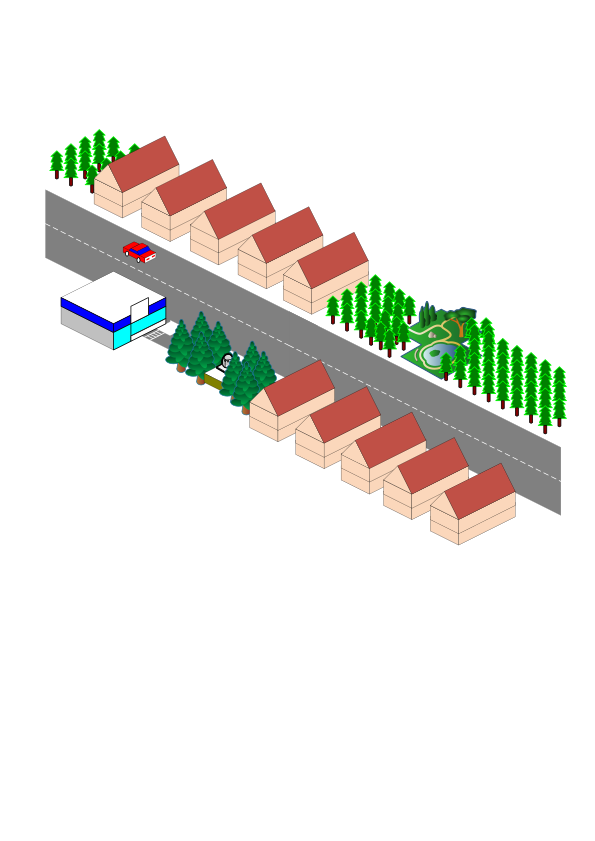
\includegraphics[scale=0.90]{../img/Dibujo1.png}
		\caption{Plano general de la urbanización}
	\end{figure}


\begin{landscape}
	\begin{figure}[H]
		\centering
		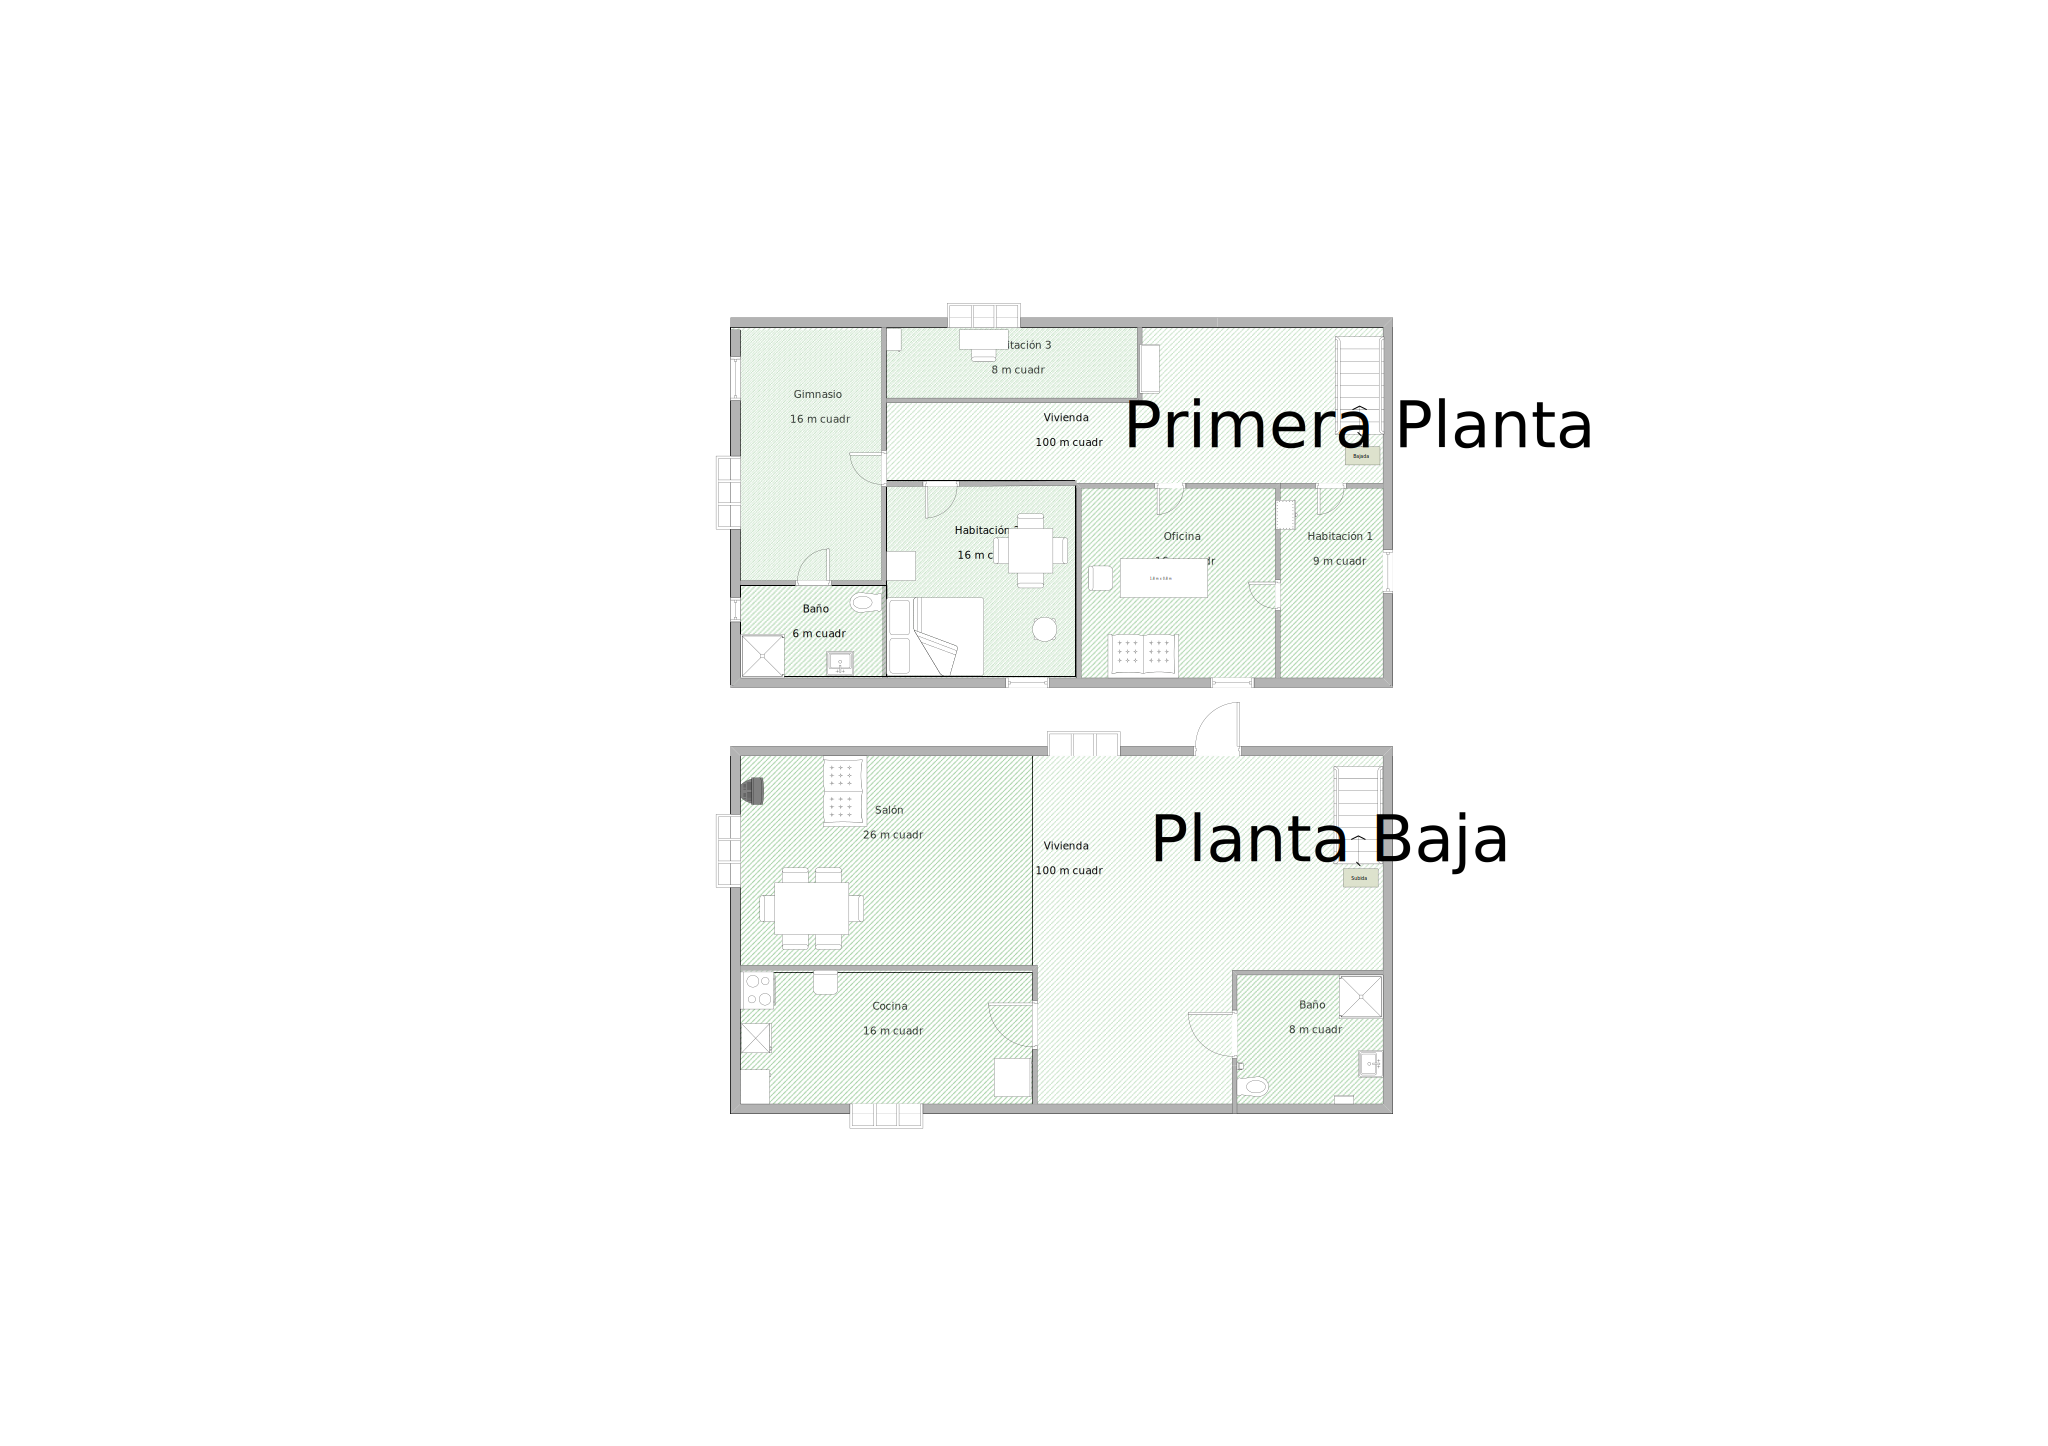
\includegraphics[scale=0.80]{../img/PlanoVivienda.png}
		\caption{Plano de la primera planta}
	\end{figure}
\end{landscape}

\begin{landscape}
	\begin{figure}[H]
		\centering
		\includegraphics[scale=0.80]{../img/PlanoVivienda2.png}
		\caption{Plano de la segunda planta}
	\end{figure}
\end{landscape}

\begin{landscape}
	\begin{figure}[H]
		\centering
		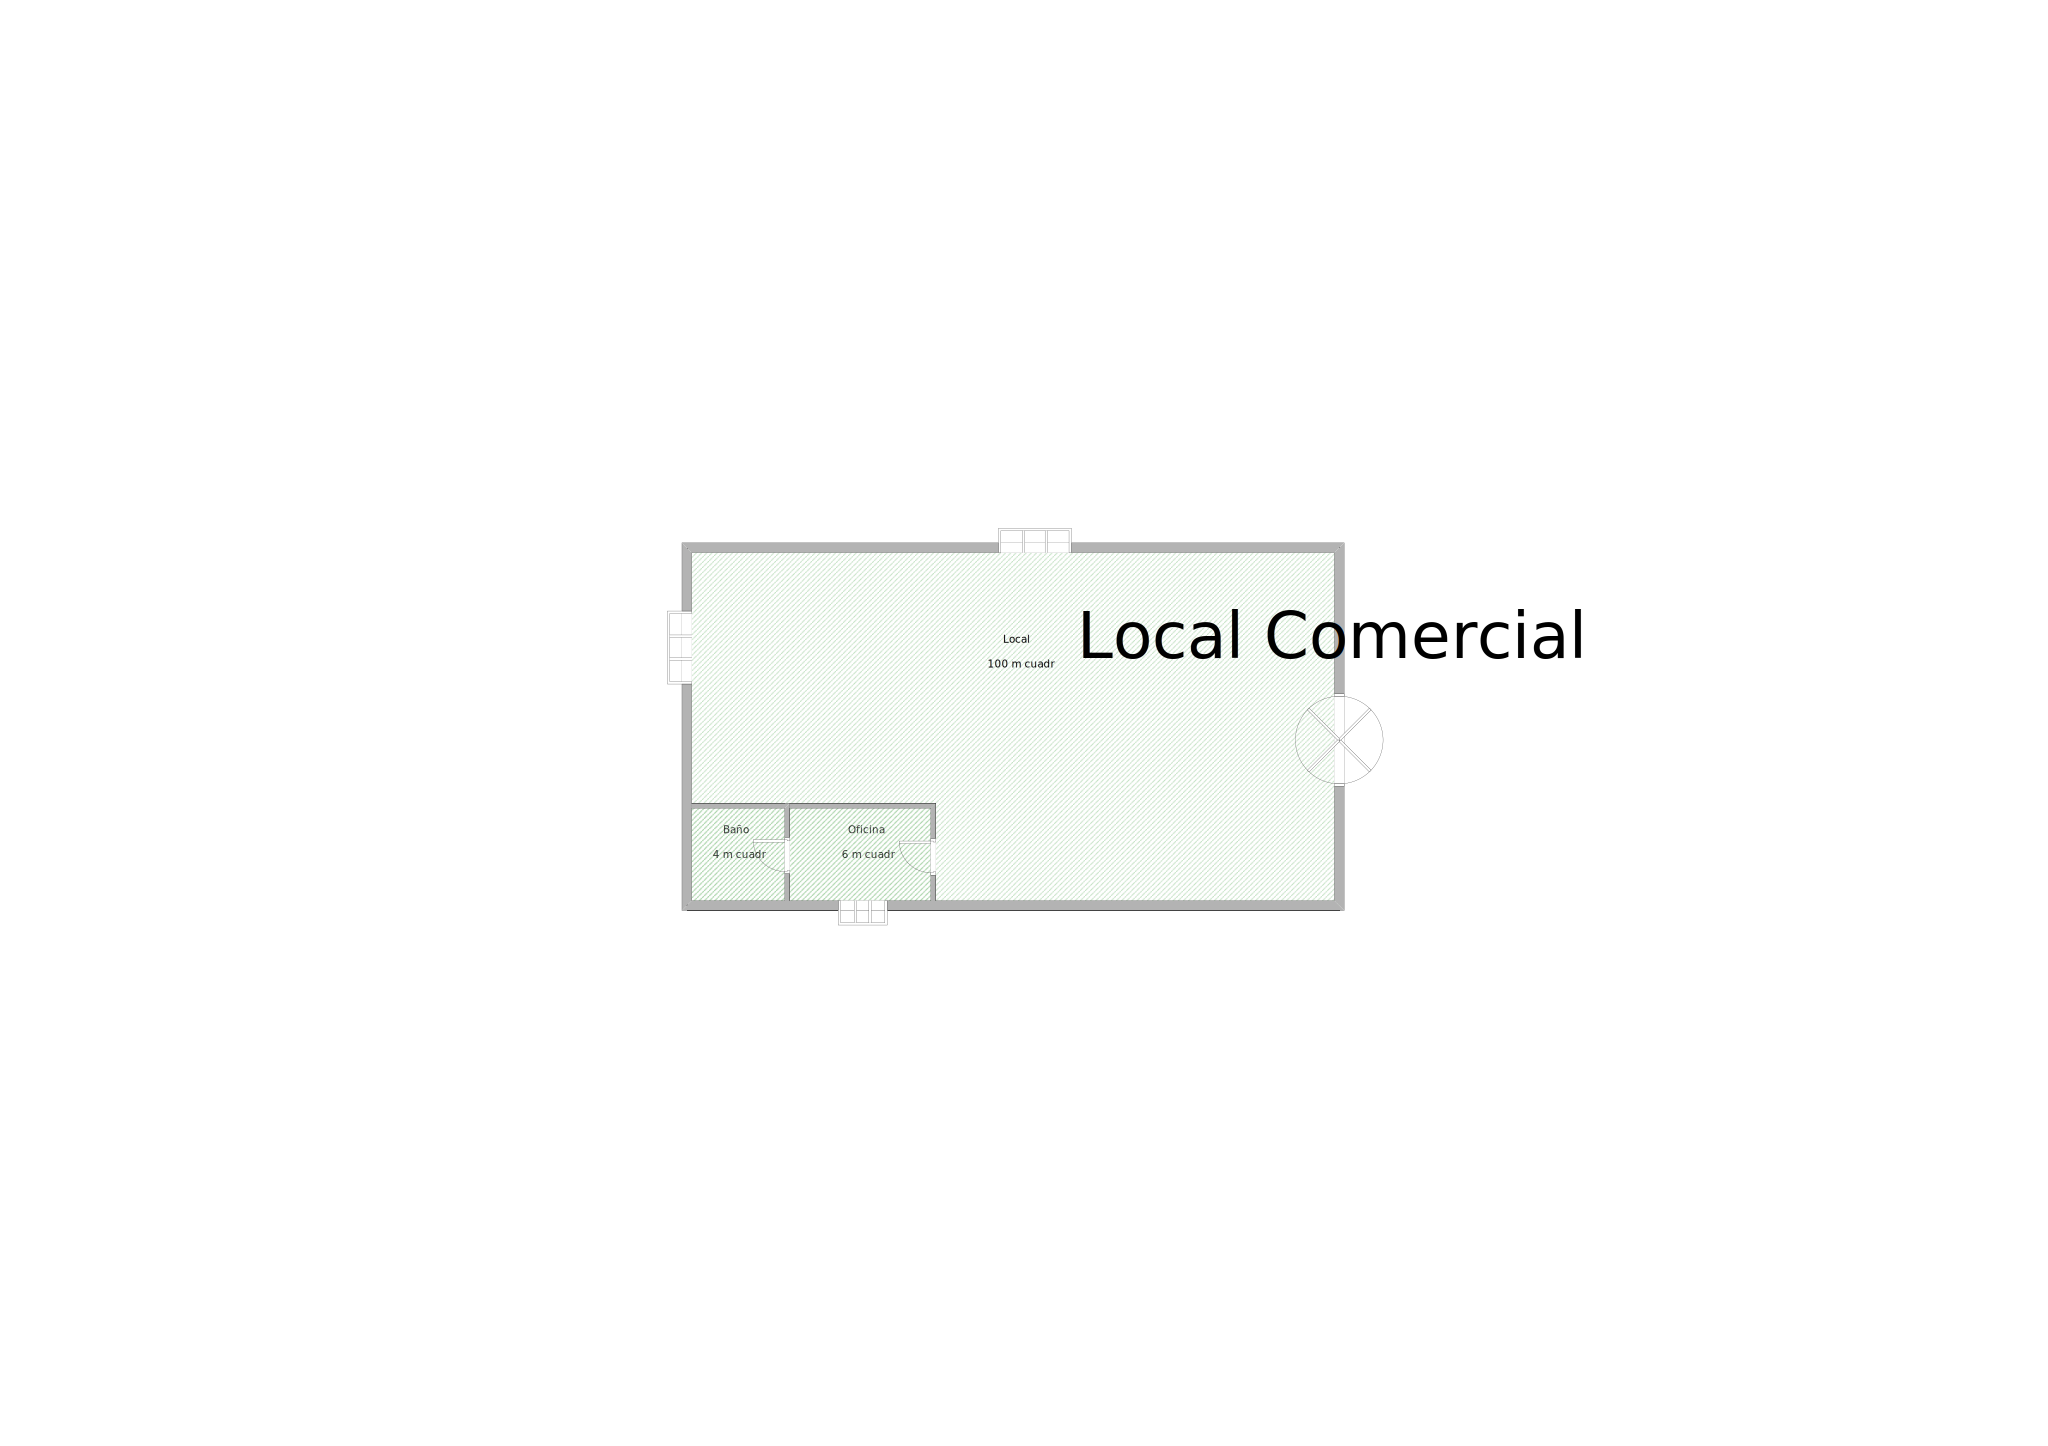
\includegraphics[scale=0.90]{../img/PlanoLocal.png}
		\caption{Plano del local comercial}
	\end{figure}
\end{landscape}

\begin{landscape}
	\begin{figure}[H]
		\centering
		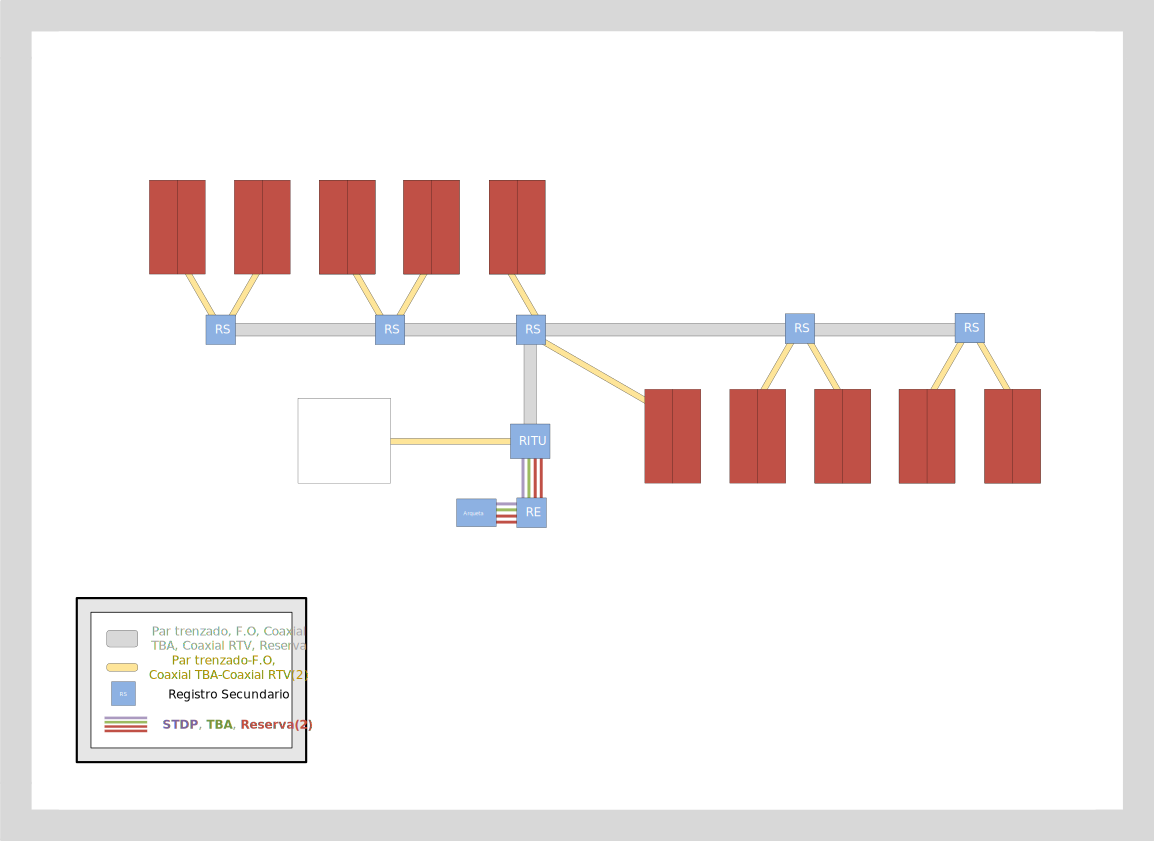
\includegraphics[scale=0.50]{../img/PLANOFINAL.pdf}
		\caption{Plano general de la instalación}
		\label{pla_general}
	\end{figure}
\end{landscape}

\begin{landscape}
	\begin{figure}[H]
		\centering
		\includegraphics[scale=0.68]{../img/PlanoCableadoVivienda1.png}
		\caption{Plano de la primera planta con cableado}
	\end{figure}
\end{landscape}

\begin{landscape}
	\begin{figure}[H]
		\centering
		\includegraphics[scale=0.68]{../img/PlanoCableadoVivienda2.png}
		\caption{Plano de la segunda planta con cableado}
	\end{figure}
\end{landscape}

\chapter{PLIEGO DE CONDICIONES.}

\section{CONDICIONES PARTICULARES.}

\subsection{Radiodifusión sonora y televisión.}
\subsubsection{Condicionantes de acceso a los sistemas de captación.}
\subsubsection{Características de los sistemas de captación.}
\paragraph{Antenas.}
\paragraph{Elementos de sujeción de las antenas para televisión terrestre.}
\paragraph{Elementos de sujeción de las antenas para televisión por satélite}
\subsubsection{Características de los elementos activos.}
\subsubsection{Características de los elementos pasivos.}
\paragraph{Mezclador.}
\paragraph{Derivadores.}
\paragraph{Distribuidores.}
\paragraph{Cables.}
\paragraph{Punto de acceso al usuario.}
\paragraph{Bases de acceso de terminal.}

\subsection{Distribución de los servicios de telecomunicaciones de telefonía disponible al público (STDP) y de banda ancha (TBA).}
\subsubsection{Redes de cables de pares o pares trenzados.}
\paragraph{Características de los cables.}
\paragraph{Características de los elementos activos.}
\paragraph{Características de los elementos pasivos.}
\subsubsection{Redes de cables coaxiales.}
\paragraph{Características de los cables.}
\paragraph{Características de los elementos pasivos.}
\subsubsection{Redes de cables de fibra óptica.}
\paragraph{Características de los cables.}
\paragraph{Características de los elementos pasivos.}
\paragraph{Características de los empalmes de fibra en la instalación.}

\subsection{Infraestructura de hogar digital.}



\chapter{PRESUPUESTO.}

\section{Infraestructura y Redes de Alimentación, Distribución y Dispersión}

\subsection{Red de RTV}

\subsubsection{Captación de señales RTV}


\begin{tabularx}{\textwidth}{lbss}

Ud. & Concepto & P. Unitario & Subtotal \\ \hline \hline
1 & Antena FM & 18,4 & 18,4 \\ \hline
1 & Antena VHF DAB & 19,2 & 19,2 \\ \hline
1 & Antenas UHF B-IV y  V (C21 a 69) & 59,8 & 59,8 \\ \hline
2 & Antena Televisión Satélite+LNB & 30 & 60 \\ \hline
1 & Mástil 3 m. & 25,65 & 25,65 \\ \hline
1 & Torreta autoestable de 3 m. & 121,24 & 121,24 \\ \hline
1 & Base para torreta. & 16,7 & 16,7 \\ \hline
20 & Mt. Cable coaxial tipo C1 & 0,75 & 15 \\ \hline
1 & Pequeño material (Tornillos, tuercas, grapas, etc...) & 14 & 14 \\ \hline
10 & Mts. Cable tierra de 25 mm2. & 2 & 20 \\ \hline
1 & Instalación de base de torreta. Ubicación y orientación de antenas en mástil y tendido y conexionado de cableado entre antenas y sistema de cabecera en RITU & 128,5 & 128,5 \\ \hline \hline
 &  & Total & 498,49 \\ 
\end{tabularx}


\subsubsection{Cabecera RTV}

\begin{tabularx}{\textwidth}{lbss}

Ud. & Concepto & P. Unitario & Subtotal \\ \hline \hline
1 & Amp. Monocanal para FM & 52,85 & 52,85 \\ \hline
8 & Amp. Monocanal para UHF (C33, C39, C49, C50, C55, C58, C59, C63) & 73,75 & 590 \\ \hline
1 & Amp. De grupo para DAB (C8 a C11) & 62,65 & 62,65 \\ \hline
1 & Amplificador de grupo C66 a C69 & 80,6 & 80,6 \\ \hline
2 & Fuente de Alimentación, 750 mA. & 78,85 & 157,7 \\ \hline
1 & Distribuidor 2 salidas. & 6,35 & 6,35 \\ \hline
2 & Mezcclador TIPO 1 para la vezcla con TVSAT & 3,4 & 6,8 \\ \hline
2 & Chasis soporte para monocanales y fuente. & 13,85 & 27,7 \\ \hline
18 & Puentes de interconexión & 2,7 & 48,6 \\ \hline
4 & Cargas adaptadoras & 0,8 & 3,2 \\ \hline
1 & Istalación de sistema de cabecera en RITU. Ajuste de amplificación e instalación de elementos pasivos de mezcla a la salida para inserción de FI & 102,8 & 102,8 \\ \hline \hline
 &  & Total & 1139,25 \\ 
\end{tabularx}


\subsubsection{Red de Distribución de RTV}

\begin{tabularx}{\textwidth}{lbss}

Ud. & Concepto & P. Unitario & Subtotal \\ \hline \hline
5 & Derivadores & 13,95 & 69,75 \\ \hline
100 & Mt. cavle tipo C1 & 0,75 & 75 \\ \hline
2 & Resistencia adaptadora 75 ohmios. & 0,06 & 0,12 \\ \hline
1 & Material para fijación & 0,6 & 0,6 \\ \hline
1 & Tendido de cableado de red de distribución para la canalización principal. Colocación de elementos pasivos, carga y adaptación de red. & 154,2 & 154,2 \\ \hline \hline
&  & Total & 299,67 \\ 
\end{tabularx}


\subsubsection{Red de Dispersión de RTV}

\begin{tabularx}{\textwidth}{lbss}

Ud. & Concepto & P. Unitario & Subtotal \\ \hline \hline
110 & Metros cable tipo C1, desde RS a RTR & 0,55 & 60,5 \\ \hline
40 & Resistencias de 75 ohmios & 0,06 & 2,4 \\ \hline
1 & Material para fijación & 0,57 & 0,57 \\ \hline
1 & Tendido y conexionado de cableado de la red de dispersión formada por cable coaxial desde el Registro Secundario hasta el RTR en el interior de cada una de las viviendas y locales. & 411 & 411 \\ \hline
\hline
&  & Total & 474,47 \\ 
\end{tabularx}

\subsection{Red de Cable Trenzado}

\subsubsection{Red de Distribución y de Dispersión. Punto de Interconexión}


\begin{tabularx}{\textwidth}{lbss}

Ud. & Concepto & P. Unitario & Subtotal \\ \hline \hline
465 & Metros de Cable de 4 pares UTP & 0,87 & 404,55 \\ \hline
1 & Panel de conexión para 24 conectores RJ45 hembra & 51,8 & 51,8 \\ \hline
19 & Conectores hembra RJ45 & 6 & 114 \\ \hline
1 & Ud. Grapas de sujeción cable en RITU en en RS & 57 & 57 \\ \hline
1 & Tendido y conexionado de la red de distribución y dispersión de cable trenzado UTP, a través de los conductos de canalización principal y secundaria, desde el Registro Principal hasta el RTR de cada vivienda y cada local. & 330 & 330 \\ \hline \hline
 &  & Total & 957,35 \\ 
\end{tabularx}

\subsection{Red de Cable Coaxial}

\subsubsection{Red de Distribución y de Dispersión. Punto de Interconexión}

\begin{tabularx}{\textwidth}{lbss}

Ud. & Concepto & P. Unitario & Subtotal \\ \hline \hline
345 & Metros de Cable Coaxial & 1,2 & 414 \\ \hline
11 & Conectores tipo F macho en extremo cable de red de distribución & 0,5 & 5,5 \\ \hline
1 & Tendido y conexionado de la red de distribución y dispersión de cable coaxial, a través de los conductos de canalización principal y secundaria, desde el Registro Principal hasta el RTR de cada vivienda y cada local. & 620 & 620 \\ \hline \hline
&  & Total & 1039,5 \\ 
\end{tabularx}

\subsection{Red de Fibra Óptica}

\subsubsection{Red de Distribución y de Dispersión. Punto de Interconexión}

\begin{tabularx}{\textwidth}{lbss}

Ud. & Concepto & P. Unitario & Subtotal \\ \hline \hline
465 & Metros de Cable de dos FO monomodo & 1,2 & 558 \\ \hline
8 & Cajas de segregación en registro secundario para contener las fibras ópticas de reserva. & 25,2 & 201,6 \\ \hline
1 & Panel de conexión para 24 conexiones dobles con sus acopladores SC/APC & 120 & 120 \\ \hline
38 & Conector SC/APC & 2,64 & 100,32 \\ \hline
1 & Tendido y conexionado de la red de distribución y dispersión de cable de fibra óptica, a través de los conductos de canalización principal y secundaria, desde el Registro Principal hasta el RTR de cada vivienda y local. & 750 & 750 \\ \hline \hline
 &  & Total & 1729,92 \\ 
\end{tabularx}

\subsection{Infraestructuras}

\subsubsection{Infraestructuras para Redes de Alimentación}

\paragraph{RTV}

\subparagraph{Armario para proteger equipos para RTV}

\begin{tabularx}{\textwidth}{lbss}

Ud. & Concepto & P. Unitario & Subtotal \\ \hline \hline
1 & Armario conforme la norma UNE20541 o UNE EN50298 y con grado de protección según las normas UNE EN60529 o UNE EN50102 & 126,81 & 126,81 \\ \hline
1 & Pequeño material (tirafondos, tacos, etc...) & 1,26 & 1,26 \\ \hline
1 & Instalación de Registro principal de RTV en RITU. & 12,85 & 12,85 \\ \hline \hline
 &  & Total & 140,92 \\ 
\end{tabularx}

\subparagraph{Anclaje Bases de Sistemas de Captación RTV}

\begin{tabularx}{\textwidth}{lbss}

Ud. & Concepto & P. Unitario & Subtotal \\ \hline \hline
2 & Base de antena parabólica compuesta por placa metálica de 250x250x2mm y cuatro zarpas varilla M16 & 77,83 & 155,66 \\ \hline
1 & Material de sujeción & 12,83 & 12,83 \\ \hline
1 & Instalación de base de parábola en cubierta del RITU. & 25,7 & 25,7 \\ \hline \hline
 &  &Total & 194,19 \\ 
\end{tabularx}


\paragraph{Infraestructuras para Redes de Operadores}

\subparagraph{Arqueta de Entrada}

\begin{tabularx}{\textwidth}{lbss}

Ud. & Concepto & P. Unitario & Subtotal \\ \hline \hline
1 & Arqueta de entrada de 400x400x600 mm de hormigón con cerco y tapa de fundición Ductil. & 294,18 & 294,18 \\ \hline
1 & Colocación y fijación de arqueta de entrada a la infraestructura común en zona de dominio público exterior a cargo de peón especializado. Excavación manual de hueco 0,193 m3, retirada de tierra y colocación de relleno. & 154,2 & 154,2 \\ \hline \hline
 &  & Total & 448,38 \\ 
\end{tabularx}

\subparagraph{Canalización Externa y Registro de Enlace Inferior}

\begin{tabularx}{\textwidth}{lbss}

Ud. & Concepto & P. Unitario & Subtotal \\ \hline \hline
0,5 & M3 de hormigón de relleno H-50 T/Max 18-20mm & 57 & 28,5 \\ \hline
25 & Mts. Tubo de material plástico no propagador de la llama, rígido diámetro 63, norma UNE 50086 con hilo guía. & 1,9 & 47,5 \\ \hline
1 & Registro  de enlace 45x45x12 cm según normativa. & 74,57 & 74,57 \\ \hline
10 & Separadores de tubos diámetro 63 mm.. & 1,2 & 12 \\ \hline
1 & Instalación de conductos para canalización entre arqueta de entrada y punto de entrada general.  & 100 & 100 \\ \hline \hline
 &  & Total & 262,57 \\ 
\end{tabularx}


\subparagraph{Registro Principal de Cable Trenzado}

\begin{tabularx}{\textwidth}{lbss}

Ud. & Concepto & P. Unitario & Subtotal \\ \hline \hline
1 & Armario conforme a la norma UNE20541 o UNE EN50298 y con grado de protección según las normas UNE EN 60529 o UNE EN 50102 & 120,8 & 120,8 \\ \hline
1 & Material de sujeción (tirafondos y tacos) & 1,26 & 1,26 \\ \hline \hline
 &  & Total & 122,06 \\ 
\end{tabularx}

\subparagraph{Registro Principal de Cable de FO}

\begin{tabularx}{\textwidth}{lbss}

Ud. & Concepto & P. Unitario & Subtotal \\ \hline \hline
1 & Armario conforme a la norma UNE20541 o UNE EN50298 y con grado de protección según las normas UNE EN 60529 o UNE EN 50102 & 120,8 & 120,8 \\ \hline
1 & Material de sujeción (tirafondos y tacos) & 1,26 & 1,26 \\ \hline \hline
 &  & Total & 122,06 \\ 
\end{tabularx}

\paragraph{Infraestructuras para Redes de Distribución y Dispersión}

\subparagraph{Canalización Principal}

\begin{tabularx}{\textwidth}{lbss}

Ud. & Concepto & P. Unitario & Subtotal \\ \hline \hline
110 & Mts. Tubo de material plástico no propagador de la llama, rígido de 50 mm  de diámetro, norma UNE50086. & 1,58 & 173,8 \\ \hline
6 & Ud. 2 bastidores soporte de tubos & 7,21 & 43,26 \\ \hline
5 & Caja registro secundario 45x45x15 cm. & 133,26 & 666,3 \\ \hline
1 & Instalación de conductos de canalización principal. & 102,8 & 102,8 \\ \hline \hline
&  & Total & 986,16 \\ 
\end{tabularx}

\subparagraph{Canalización Secundaria}

\begin{tabularx}{\textwidth}{lbss}

Ud. & Concepto & P. Unitario & Subtotal \\ \hline \hline
165 & Mts. De tubo de 25mm de material plástico no propagador de la llama, rígido, norma UNE50086. & 0,66 & 108,9 \\ \hline
1 & Instalación de conductos que componen la canalización secundaria. & 346,5 & 346,5 \\ \hline \hline
 &  & Total & 455,4 \\ 
\end{tabularx}

\paragraph{Recintos de Instalaciones de Telecomunicación}

\begin{tabularx}{\textwidth}{lbss}

Ud. & Concepto & P. Unitario & Subtotal \\ \hline \hline
1 & Armario de 2000x1500x500 mm (RITU) & 874,74 & 874,74 \\ \hline
1 & Instalación de Recinto de Instalación de comunicaciones Único. & 51,4 & 51,4 \\ \hline \hline
 &  & Total & 926,14 \\ 
\end{tabularx}

\paragraph{Resumen parte 1. Infraestructura y Redes de Alimentación, Distribución y Dispersión}

\begin{center}
\begin{tabular}{l r}

Partida 1.1.-  Red de RTV & 2411,88 \\ 
Partida 1.2.- R. Cable Trenzado & 957,35 \\ 
Partida 1.3.- R. Coaxial & 1039,5 \\ 
Partida 1.4.- R. FO & 1729,92 \\ 
Partida 1.5.- Infraestructuras & 3657,88 \\  \hline
Total & 9796,53 \\ 
\end{tabular}
\end{center}

\section{Infraestructura y Redes Interiores de Usuario}

\subsection{Red Interior RTV}

\subsubsection{Punto de Acceso de Usuario RTV}

\begin{tabularx}{\textwidth}{lbss}
Ud. & Concepto & P. Unitario & Subtotal \\ \hline \hline
11 & PAU RTV con conector tipo F a su entrada. & 6,3 & 69,3 \\ \hline
20 & Conector tipo F & 0,5 & 10 \\ \hline
10 & Distribuidor con 7 salidas transparentes en 5-2.150 MHz & 9,95 & 99,5 \\ \hline
22 & Resistencias 75 ohmios tipo F & 0,4 & 8,8 \\ \hline
1 & Pequeño material para fijación de mecanismos en registro. & 0,6 & 0,6 \\ \hline
1 & Instalación de equipos pasivos de terminación, paso y distribución de señales de RTV distribuidas en la ICT. Fijación a fondo de Registro de Terminación de Red y conectorización y conexionado del cableado al dispositivo PAU. & 154,2 & 154,2 \\ \hline \hline
 &  & Total & 342,4 \\ 
\end{tabularx}

\subsubsection{Toma de Usuario y Red de Usuario de RTV}

\begin{tabularx}{\textwidth}{lbss}
Ud. & Concepto & P. Unitario & Subtotal \\ \hline \hline
70 & Tomas de RTV, transparentes 5-2.150 MHz & 7,3 & 511 \\ \hline
70 & Embellecedor TV-FM/FI & 0,7 & 49 \\ \hline
70 & Conector tipo F & 0,5 & 35 \\ \hline
450 & Mt. cable coaxial tipo C1, desde RTR a toma & 0,75 & 337,5 \\ \hline
1 & Tendido de cableado interior desde PAU de distribución de RTV hasta las tomas de servicio de RTV. Instalación de tomas de servicio de radiodifusión sonora y televisión en el interior de cada una de las viviendas. Conexión del cableado procedente de la distribución del PAU, colocación del embellecedor y comprobación de niveles. & 1953,29 & 1953,29 \\ \hline \hline
 &  & Total & 2885,79 \\ 
\end{tabularx}

\subsection{Red Interior Cable Trenzado}

\subsubsection{Punto de Acceso de Usuario de Red de Cable Trenzado}

\begin{tabularx}{\textwidth}{lbss}
Ud. & Concepto & P. Unitario & Subtotal \\ \hline \hline
11 & Roseta de terminación de red & 6,83 & 75,13 \\ \hline
11 & Conector RJ45 hembra. & 6 & 66 \\ \hline
10 & Multiplexores pasivos de 7 salidas. & 5,4 & 54 \\ \hline
10 & Latiguillos cat. 6 & 10,5 & 105 \\ \hline
1 & Pequeño material para fijación de mecanismos en registro. & 0,42 & 0,42 \\ \hline
1 & Instalación y conexionado de roseta de terminación de red de cable de pares trenzados. & 350,33 & 350,33 \\ \hline \hline
&  & Total & 650,88 \\ 
\end{tabularx}

\subsubsection{Toma de Usuario y Red de Cable Trenzado}

\begin{tabularx}{\textwidth}{lbss}
Ud. & Concepto & P. Unitario & Subtotal \\ \hline \hline
90 & Toma RJ45 con embellecedor. & 8,5 & 765 \\ \hline
90 & Conectores macho RJ45  en RTR. & 6,23 & 560,7 \\ \hline
480 & Mts. Cable de cobre de 4 pares UTP categoría 6, libre de halógenos desde RTR a toma de usuario. & 0,7 & 336 \\ \hline
1 & Ud. Material de sujeción. & 0,14 & 0,14 \\ \hline
1 & Tendido de cableado horizontal desde Registro de Terminación de red hasta cada una de las tomas RJ45 de servicio en el interior de las viviendas. Instalación de rosetas RJ45, inserción de pares y comprobación. & 1426,35 & 1426,35 \\ \hline \hline
 &  & Total & 3088,19 \\ 
\end{tabularx}

\subsection{Red Interior Cable Coaxial}

\subsubsection{Punto de Acceso de Usuario de Red de Cable Coaxial}

\begin{tabularx}{\textwidth}{lbss}
Ud. & Concepto & P. Unitario & Subtotal \\ \hline \hline
11 & Distribuidores de dos salidas. & 6,9 & 75,9 \\ \hline
11 & Conector tipo F macho, entrada a distribuidor. & 0,5 & 5,5 \\ \hline
11 & Resistencias 75 ohmios tipo F en distribuidor. & 0,4 & 4,4 \\ \hline
1 & Pequeño material para fijación de mecanismos en registro. & 0,42 & 0,42 \\ \hline
1 & Instalación y conexionado del distribuidor de dos salidas. & 120 & 120 \\ \hline \hline
 &  & Total & 206,22 \\ 
\end{tabularx}

\subsubsection{Toma de Usuario y Red de Cable Coaxial}

\begin{tabularx}{\textwidth}{lbss}
Ud. & Concepto & P. Unitario & Subtotal \\ \hline \hline
70 & Toma coaxial con embellecedor. & 8,2 & 574 \\ \hline
70 & Conector tipo F macho, salida de distribuidor. & 0,5 & 35 \\ \hline
450 & Mts. Cable coaxial libre de halógenos desde RTR a toma. & 0,7 & 315 \\ \hline
1 & Ud. Material sujeción. & 0,14 & 0,14 \\ \hline
1 & Tendido de cableado horizontal desde Registro de Terminación de Red hasta cada una de las tomas de usuario en el interior de las viviendas. & 1525,5 & 1525,5 \\ \hline \hline
 &  & Total & 2449,64 \\ 
\end{tabularx}

\subsection{Punto de Terminación de Red de FO}

\subsubsection{Punto de Acceso de Usuario de Red de FO}

\begin{tabularx}{\textwidth}{lbss}
Ud. & Concepto & P. Unitario & Subtotal \\ \hline \hline
11 & Roseta de terminación de red con dos acopladores. & 15 & 165 \\ \hline
22 & Conector SC/APC & 2,64 & 58,08 \\ \hline
1 & Pequeño material para fijación de macanismos en registro. & 0,42 & 0,42 \\ \hline
1 & Instalación y conexionado de roseta de terminación de red de fibra óptica. & 385,5 & 385,5 \\ \hline \hline
 &  &  Total & 609 \\ 
\end{tabularx}

\subsection{Infraestructuras}

\subsubsection{Canalización Interior de RTV}

\begin{tabularx}{\textwidth}{lbss}
Ud. & Concepto & P. Unitario & Subtotal \\ \hline \hline
450 & Mts. Tubo de material plástico no propagador de la llama, corrugado de 20 mm  de diámetro. & 0,33 & 148,5 \\ \hline
70 & Cajas registro de toma (64x64x42)mm. & 0,54 & 37,8 \\ \hline
1 & Tendido de conductos de unión del Registro de Terminación de Red y los diferentes registros destinados a la instalación de tomas de servicio RTV en cada una de las viviendas. & 1233,6 & 1233,6 \\ \hline \hline
 &  & Total & 1419,9 \\ 
\end{tabularx}

\subsubsection{Canalización Interior de Cable Trenzado}

\begin{tabularx}{\textwidth}{lbss}
Ud. & Concepto & P. Unitario & Subtotal \\ \hline \hline
480 & Mts. Tubo de material plástico no propagador de la llama, corrugado de 20mm de diámetro. & 0,33 & 158,4 \\ \hline
90 & Cajas registro de toma (64x64x42) mm. & 0,54 & 48,6 \\ \hline
1 & Tendido de conductos de unión del Registro de Terminación de Red y los diferentes registros destinados a la instalación de tomas de servicio RJ45 en cada una de las viviendas.  & 1737,85 & 1737,85 \\ \hline \hline
 &  & Total & 1944,85 \\ 
\end{tabularx}

\subsubsection{Canalización Interior de Coaxial}

\begin{tabularx}{\textwidth}{lbss}
Ud. & Concepto & P. Unitario & Subtotal \\ \hline \hline
450 & Mts. Tubo de material plástico no propagador de la llama, corrugado de 20 mm de diámetro. & 0,33 & 148,5 \\ \hline
1 & Tendido y fijación de conductos de unión entre Registro de Terminación de Red y los diferentes registros de Cable Coaxial. & 330 & 330 \\ \hline
50 & Cajas de registro de toma & 0,54 & 27 \\ \hline \hline
 &  & Total & 505,5 \\ 
\end{tabularx}

\subsubsection{Registros de Terminación de Red y Registros de Toma Configurable}

\begin{tabularx}{\textwidth}{lbss}
Ud. & Concepto & P. Unitario & Subtotal \\ \hline \hline
11 & Cajas Registro de Terminación de red de 500x600x80 mm & 40,26 & 442,86 \\ \hline
10 & Mts tubo de material plástico no propagador de la llama, corrugado de 20 mm de diámetro, con hilo guía. & 0,33 & 3,3 \\ \hline
10 & Cajas Registros de Toma configurable 64x64x42 mm & 0,54 & 5,4 \\ \hline
1 & Instalación de Registros de Terminación de Red en el interior de las viviendas y locales. Fijación en fondo de tabique seco en la ubicación señalada en proyecto. Tendido y fijación de conductos de unión entre Registro de Terminación de Red y los registros configurables. & 102,8 & 102,8 \\ \hline \hline
 &  & Total & 554,36 \\ 
\end{tabularx}

\subsubsection{Registros de Paso}

\begin{tabularx}{\textwidth}{lbss}
Ud. & Concepto & P. Unitario & Subtotal \\ \hline \hline
40 & Cajas Registro de Paso (100x160x40) mm & 20,5 & 820 \\ \hline
1 & Instalación de Registros de Paso en el interior de las viviendas en la ubicación señalada en proyecto. & 242,4 & 242,4 \\ \hline \hline
 &  &  Total & 1062,4 \\ 
\end{tabularx}

\paragraph{Resumen parte 2. Infraestructura y Redes Interiores de Usuario}

\begin{center}
\begin{tabular}{l r}
\hline
Partida 2.1.- Red Interior RTV & 3228,19 \\ 
P 2.2.- R.I. Cable Trenzado & 3739,07 \\ 
P 2.3.- R.I. Cable Coaxial & 2655,86 \\ 
P 2.4.- PTR fibra Optica & 609 \\ 
P 2.5.- Infraestructuras & 5487,01 \\ \hline
Total & 15719,13 \\ 
\end{tabular}
\end{center}

\section{Resumen}

\begin{tabularx}{\textwidth}{bs}
Total Parte 1. Infraestructura y Redes de Alimentación, Distribución y Dispersión. &  9796,53 \\
Total Parte 2. Infraestructuras y Redes Interiores de usuario & 15719,13 \\ \hline \hline
Total Proyecto & 25515,66 \\
\end{tabularx}




\end{document}
